\documentclass[12pt]{article}
\usepackage{graphicx,import}
\usepackage[svgnames]{xcolor} 
\usepackage{fancyhdr}
\usepackage{subfig}
\usepackage{hyperref}
\usepackage{enumitem}
\usepackage{cite}
\usepackage[many]{tcolorbox}
\usepackage{listings }
\usepackage[a4paper, total={6in, 8in} , bottom = 25mm , top = 25mm, headheight = 1.25cm , includehead,includefoot,heightrounded ]{geometry}
\usepackage{afterpage}
\usepackage{amssymb}
\usepackage{pdflscape}
\usepackage{gensymb}
\usepackage{textcomp}
\usepackage{tikz,pgfplots}
\usepackage{xecolor}
\usepackage{rotating}
\usepackage{pdfpages}
\usepackage{fancyvrb}
\usepackage[Kashida]{xepersian}
\usepackage[T1]{fontenc}
\usepackage{tikz}
\usepackage[utf8]{inputenc}
\usepackage{PTSerif} 
\usepackage{seqsplit}

\usepackage[edges]{forest}

\usepackage{listings}
\usepackage{xcolor}

\hypersetup{
	colorlinks   = true, %Colours links instead of ugly boxes
	urlcolor     = blue, %Colour for external hyperlinks
	linkcolor    = blue, %Colour of internal links
	citecolor   = red %Colour of citations
}

\definecolor{codegreen}{rgb}{0,0.6,0}
\definecolor{codegray}{rgb}{0.5,0.5,0.5}
\definecolor{codepurple}{rgb}{0.58,0,0.82}
\definecolor{backcolour}{rgb}{0.95,0.95,0.92}

\NewDocumentCommand{\codeword}{v}{
	\texttt{\textcolor{blue}{#1}}
}
\lstset{language=java,keywordstyle={\bfseries \color{blue}}}

\lstdefinestyle{mystyle}{
	backgroundcolor=\color{backcolour},   
	commentstyle=\color{codegreen},
	keywordstyle=\color{magenta},
	numberstyle=\tiny\color{codegray},
	stringstyle=\color{codepurple},
	basicstyle=\ttfamily\normalsize,
	breakatwhitespace=false,         
	breaklines=true,                 
	captionpos=b,                    
	keepspaces=true,                 
	numbers=left,                    
	numbersep=5pt,                  
	showspaces=false,                
	showstringspaces=false,
	showtabs=false,                  
	tabsize=2
}

\lstset{style=mystyle}

\settextfont[Scale=1.2 ,BoldFont={Bahij Nazanin-Bold.ttf} , ItalicFont = {IRNazaninIranic.ttf}]{Bahij Nazanin-Regular.ttf}
\setlatintextfont[Scale = 1.0]{Garamond}
\DefaultMathsDigits 
\DeclareMathSizes{11}{19}{13}{9} 
%\DeclareMathSizes{12}{14.4}{8}{9}





\newenvironment{changemargin}[2]{%
	\begin{list}{}{%
			\setlength{\topsep}{0pt}%
			\setlength{\leftmargin}{#1}%
			\setlength{\rightmargin}{#2}%
			\setlength{\listparindent}{\parindent}%
			\setlength{\itemindent}{\parindent}%
			\setlength{\parsep}{\parskip}%
		}%
		\item[]}{\end{list}}


\definecolor{foldercolor}{RGB}{124,166,198}

\tikzset{pics/folder/.style={code={%
			\node[inner sep=0pt, minimum size=#1](-foldericon){};
			\node[folder style, inner sep=0pt, minimum width=0.3*#1, minimum height=0.6*#1, above right, xshift=0.05*#1] at (-foldericon.west){};
			\node[folder style, inner sep=0pt, minimum size=#1] at (-foldericon.center){};}
	},
	pics/folder/.default={20pt},
	folder style/.style={draw=foldercolor!80!black,top color=foldercolor!40,bottom color=foldercolor}
}

\forestset{is file/.style={edge path'/.expanded={%
			([xshift=\forestregister{folder indent}]!u.parent anchor) |- (.child anchor)},
		inner sep=1pt},
	this folder size/.style={edge path'/.expanded={%
			([xshift=\forestregister{folder indent}]!u.parent anchor) |- (.child anchor) pic[solid]{folder=#1}}, inner xsep=0.6*#1},
	folder tree indent/.style={before computing xy={l=#1}},
	folder icons/.style={folder, this folder size=#1, folder tree indent=3*#1},
	folder icons/.default={12pt},
}

\begin{document}
	
	
	%%% title pages
	\begin{titlepage}
		\begin{center}
			
			\vspace*{0.7cm}
			
			
\includegraphics[width=0.4\textwidth]{sharif1.png}\\
			\vspace{0.5cm}
			\textbf{ \Huge{\emph  ﺷﺒﻜﻪ‌های کامپیوتری} }\\
			\vspace{0.5cm}
			\textbf{ \Large{ تمرین دوم} }
			\vspace{0.2cm}
			
			
			\large \textbf{دانشکده مهندسی کامپیوتر}\\\vspace{0.2cm}
			\large   دانشگاه صنعتی شریف\\\vspace{0.2cm}
			\large   ﻧﯿﻢ سال دوم 00-99 \\\vspace{0.2cm}
			\noindent\rule[1ex]{\linewidth}{1pt}
			استاد:\\
			\textbf{{جناب آقای دکتر جعفری}}
			
			
			\vspace{0.15cm}
			نام و نام خانوادگی:\\
			
			
			\textbf{{امیرمهدی نامجو - 97107212}}
		\end{center}
	\end{titlepage}
	%%% title pages
	
	
	%%% header of pages
	\newpage
	\pagestyle{fancy}
	\fancyhf{}
	\fancyfoot{}
	\cfoot{\thepage}
	\chead{تمرین دوم}
	\rhead{
\includegraphics[width=0.1\textwidth]{sharif.png}}
	\lhead{امیرمهدی نامجو}
	%%% header of pages
	
	\KashidaOff
	
	\section{سوال اول}
	
	\textbf{توجه: امکان زوم بر روی تمامی تصاویری که در متن قرار دارند وجود دارد.}
	
	\begin{enumerate}
		
		\item
		
		وضعیت درخواست‌های DNS رد و بدل شده برای فیسبوک به صورت زیر است:
		
		\begin{center}
			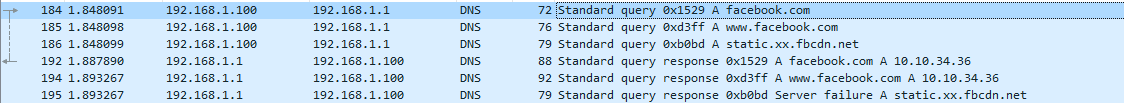
\includegraphics[width = 1.0 \textwidth]{images/1.png}
		\end{center}

سه درخواست اول از کامپیوتر من به روتر رفته‌اند و سه مورد بعدی جواب‌هایی هستند که از روتر به کامپیوتر من برگشته اند. مشاهده می‌کنیم آدرس آی‌پی که برای فیسبوک برگشته است
\lr{\Verb+10.10.34.36+}
است.

این آدرس آی‌پی جزو دسته آی‌پی‌های رزرو شده است که بین
\lr{\Verb+10.0.0.0+}
تا
\lr{\Verb+10.255.255.255+}
قرار دارد. این آدرس آی‌پی‌ها مربوط به شبکه‌های خصوصی هستند و عملا به سایت خاصی در اینترنت نگاشت نشده‌اند. این یعنی \lr{DNS} سرور، آدرسی را برای سایت \lr{Facebook} برگردانده که عملا مربوط به شبکه عمومی اینترنت نمی‌شود و یک آدرس در شبکه خصوصی است که عملا در کامپیوتر من وجود  نداشته و نتیجتا کروم با خطای
\lr {\Verb+This site can’t be reached+}
و
\lr{\Verb+ERR\_CONNECTION\_TIMED\_OUT+}
متوقف می‌شود.
	
	با بررسی تنظیمات مودم متوجه شدم که DNS-Server پیش‌فرض آن به صورت \lr{\Verb+46.224.1.220+} است که با \lr{IpLookup} کردن آن، متوجه می‌شویم که این آی‌پی متعلق به \lr{\Verb+ns5.hiweb.ir+} یعنی Nameserver «های‌وب» در ایران است و منطقی است که فیلترینگ روی این Nameserver داخلی اعمال شده باشد و در نتیجه DNS به آن نتیجه نامعتبری برای \lr{facebook.com} که یک سایت فیلتر شده است برگرداند.
	
	
	\item
	
	وضعیت درخواست DNS برای سایت اوراکل به صورت زیر است:
	
		\begin{center}
		
\includegraphics[width = 1.0 \textwidth]{images/2.png}
	\end{center}
	
	


وضعیت خروجی برگدانده شده برای آن به صورت زیر است:

\begin{latin}
	\begin{verbatim}
		Answers
		www.oracle.com: type CNAME, class IN,
		 cname ds-www.oracle.com.edgekey.net
		Name: www.oracle.com
		Type: CNAME (Canonical NAME for an alias) (5)
		Class: IN (0x0001)
		Time to live: 497 (8 minutes, 17 seconds)
		Data length: 31
		CNAME: ds-www.oracle.com.edgekey.net
		ds-www.oracle.com.edgekey.net: type CNAME, class IN,
		 cname e2581.dscx.akamaiedge.net
		Name: ds-www.oracle.com.edgekey.net
		Type: CNAME (Canonical NAME for an alias) (5)
		Class: IN (0x0001)
		Time to live: 451 (7 minutes, 31 seconds)
		Data length: 24
		CNAME: e2581.dscx.akamaiedge.net
		e2581.dscx.akamaiedge.net: type A, class IN, addr 23.14.117.40
		Name: e2581.dscx.akamaiedge.net
		Type: A (Host Address) (1)
		Class: IN (0x0001)
		Time to live: 497 (8 minutes, 17 seconds)
		Data length: 4
		Address: 23.14.117.40
		
	\end{verbatim}
\end{latin}
	
	جواب اول مشخص می‌کند که \lr{\Verb+www.oracle.com+} در اصل یک \lr{Alias} برای یک آدرس دیگر است.
	
	 جواب دوم مشخص می‌کند که آدرس مشخص شده بعدی یعنی
	 
	  \lr{\Verb+ds-www.oracle.com.edgekey.net+}
	  
	   هم یک \lr{Alias} برای آدرس دیگری است. آدرس نهایی یعنی \lr{\Verb+e2581.dscx.akamaiedge.net+} به یک آدرس آی‌پی واقعی مپ شده است. این آدرس ای‌پی یعنی \lr{\Verb+23.14.117.40+} مربوط به یکی از \lr{CDN} های شرکت \lr{Akamai} است. این \lr{CDN} در ترکیه واقع شده است و براساس موقعیت مکانی من که ایران بوده، نزدیک‌ترین \lr{CDN} تشخیص داده شده مربوط به کشور ترکیه بوده است. با این وجود در نهایت شاهد این هستیم که سایت \lr{Oracle} باز نمی‌شود و با خطاهای 
	\lr {\Verb+This site can’t be reached+}
	و
	\lr{\Verb+ERR\_CONNECTION\_TIMED\_OUT+}
	مواجه می‌شویم. این خطاها این بار به خاطر فیلترینگ نیستند بلکه به خاطر تحریم است.
	
	
		
	
	
	\item
	
	پیش از بررس نتایج باید بررسی کنیم که آی‌پی آدرس DNS-Server های شکن متعلق به کجاست. در سایت دو آی‌پی آدرس قرار گرفته است. اولین مورد \lr{\Verb+178.22.122.100+} است که متعلق به شرکت آسیاتک (\lr{Asiatech Data Transmission company}) بوده و دومین آی‌پی \lr{\Verb+185.51.200.2+} است که متعلق به شرکت مهندسی صفرویک پرداز (\lr{Sefroyek Pardaz Engineering Co. LTD}) است.
	
با انجام تنظیمات مربوطه و وارد کردن آدرس Oracle داریم:

			\begin{center}
		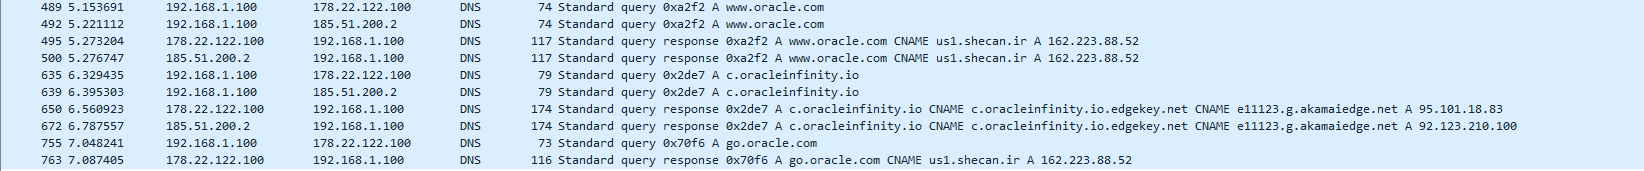
\includegraphics[width = 1.0 \textwidth]{images/3.png}
	\end{center}
	
	همان طور که در تصویر مشخص است در نتیجه درخواست آدرس \lr{\Verb+www.oracle.com+} خروجی به این صورت بوده که این آدرس Alias ای برای آدرس \lr{\Verb+us1.shecan.ir+} است و آدرس آی‌پی \lr{\Verb+162.223.88.52+} گزارش شده است. این آدرس آی‌پی در آمریکا قرار داشته و متعلق به شرکتی به اسم ColoUp است. با مراجعه به سایت این شرکت می‌توان مشاهده کرد که این شرکت مرتبط به خدمات شبکه است و البته بخش گزارش خطا به زبان فارسی هم دارد در نتیجه می‌توان به این نتیجه رسید که با شکن در ارتباط است.
			\begin{center}
		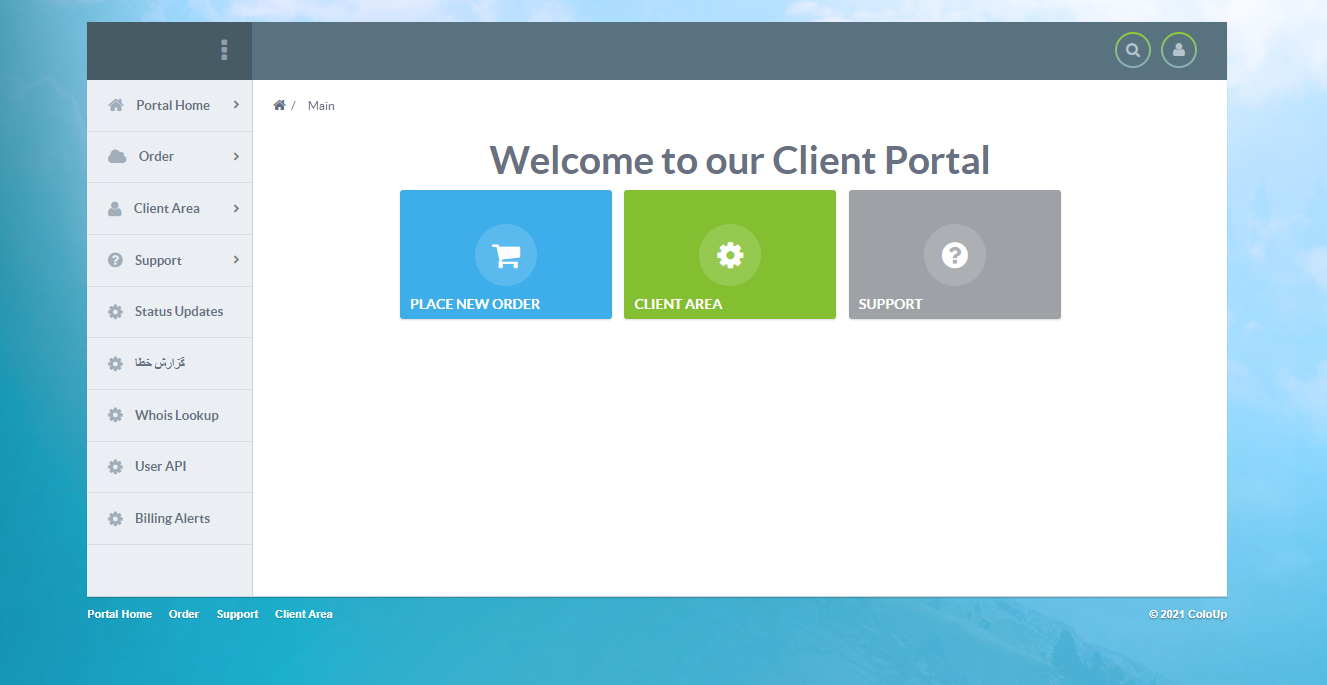
\includegraphics[width = 0.5 \textwidth]{images/4.png}
	\end{center}

خروجی برگردانده شده به صورت زیر است:

\begin{latin}
	\begin{verbatim}
		Answers
		www.oracle.com: type CNAME, class IN, cname us1.shecan.ir
		Name: www.oracle.com
		Type: CNAME (Canonical NAME for an alias) (5)
		Class: IN (0x0001)
		Time to live: 118 (1 minute, 58 seconds)
		Data length: 15
		CNAME: us1.shecan.ir
		us1.shecan.ir: type A, class IN, addr 162.223.88.52
		Name: us1.shecan.ir
		Type: A (Host Address) (1)
		Class: IN (0x0001)
		Time to live: 214 (3 minutes, 34 seconds)
		Data length: 4
		Address: 162.223.88.52
		
	\end{verbatim}
	\end{latin}

سایر موارد مربوط به \lr{Oracle} که مشاهده می‌شود، مربوط به \lr{CDN} ها و موارد متفرقه دیگری هستند که تحریم نبوده و همان \lr{IP} اصلی آن ها برگردانده شده است. البته \lr{\Verb+go.oracle.com+} هم تحریم است و برای آن هم آدرس مربوط به \lr{\Verb+ us1.shecan.ir+} برگردانده شده است.

بدین ترتیب به نظر می‌رسد که درخواست‌هایی که ما برای سایت \lr{Oracle} می‌فرستیم به جای این که مستقیما به سایت \lr{Oracle} برود، به سایت واسطه‌ای که آدرس آن \lr{\Verb+ us1.shecan.ir +} است می‌رود و سپس از طریق این سایت به \lr{Oracle} منتقل شده و جواب‌ها هم از طریق همین سایت با آی‌پی 
\lr{\Verb+ 162.223.88.52 +}
برای ما بر می‌گردد:
		\begin{center}
	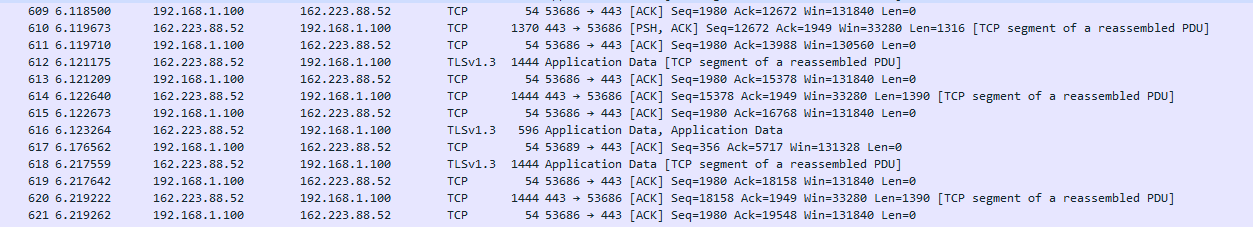
\includegraphics[width = 0.5 \textwidth]{images/5.png}
\end{center}

از آن‌جایی که این آی‌پی در آمریکا قرار دارد و درخواست‌های ما از طریق آن به \lr{Oracle} منتقل می‌شود، \lr{Oracle} تحریم را اعمال نکرده و اطلاعات را به سرورهای شکن فرستاده و از آن طریق پاسخ مربوطه به ما بر می‌گردد.

در مورد مواردی که تحریم نیستند، آدرس ای‌پی تغییری نمی‌کند و در این زمینه شکن تغییری در روند کار ایجاد نکرده و مانند یک \lr{DNS-Server} معمولی عمل می‌کند.


نتایجی که برای فیسبوک بر می‌گردد به صورت زیر است:

		\begin{center}
	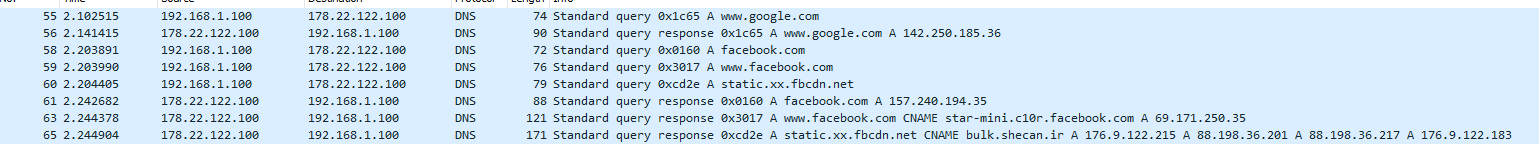
\includegraphics[width = 0.5 \textwidth]{images/6.png}
\end{center}

آی‌پی‌هایی که با آدرس‌های
\lr{\Verb+69.171.250.35+}
و
\lr{\Verb+157.240.194.35+}
برگردانده می‌شوند، هر دو واقعا متعلق به فیسبوک هستند. اما با این حال اگر پکت‌های TCP جا به جا شده به این IP را مشاهده کنیم وضعیت زیر را می‌بینیم:

		\begin{center}
	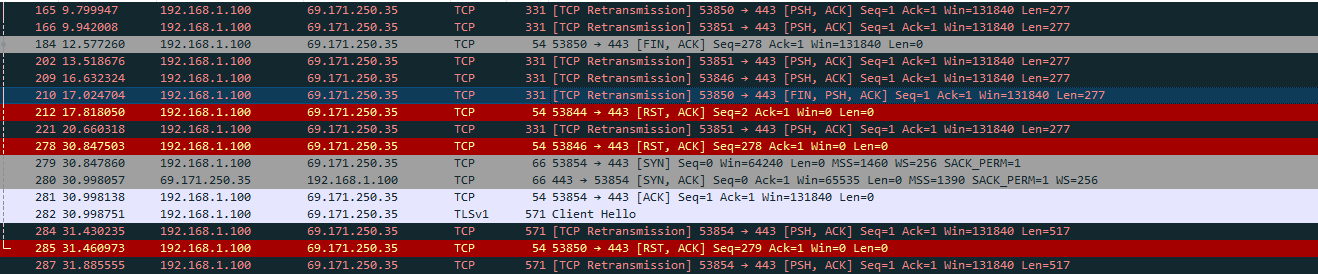
\includegraphics[width = 0.5 \textwidth]{images/7.png}
	\end{center}

مشاهده می‌شود که اکثر موارد به رنگ سیاه یا قرمز هستند. سیاه با حروف قرمز به معنی \lr{BAD TCP} و قرمز با حروف زرد به معنی \lr{TCP RST} است. تقریبا هیچ‌کدام از پکت‌های ارسالی ما به درستی به فیسبوک منتقل نشده‌اند. این بدین معنی است که فیلترینگ اعمال شده برای فیسبوک تنها در لایه \lr{DNS} نیست. بلکه فیلترینگ‌های دیگری هم اعمال شده است که پکت‌ها را بعد از رسیدن به \lr{ISP}‌های داخلی، با توجه به آدرس آن که مربوط به فیسبوک است و جزو سایت‌های فیلتر شده است، \lr{Drop} می‌کند تا به فیسبوک نرسند.

در این مورد \lr{Shecan} هم نقش خاصی ایفا نکرده و صرفا آدرس واقعی سایت \lr{\Verb+www.facebook.com+} را به ما برگردانده است و از آن‌جایی که جزو سایت‌های تحریمی هم نیست، آدرس سرورهای \lr{\Verb+us1.shecan.ir+} را به ما نداده است.


\item

خیر همان طور که در بالا توضیح داده شد، روش کار شکن بدین صورت است که لیستی از سایت‌های تحریم شده دارد و برای آن سایت‌ها، آی‌پی مربوط به سرورهای خود شکن را که در کشور دیگری مستقر هستند به ما بر می‌گرداند. بدین ترتیب، ریکوئست‌های ما به آن سایت از طریق سرورهای شکن که به نوعی نقش \lr{Man in the Middle} را ایفا کرده است به آن سایت منتقل شده و جواب‌ها از طریق این سرور شکن به ما می‌رسد.

در مورد سایت‌های فیلتر شده، شکن یا عملکردی مانند \lr{DNS} های \lr{ISP} ها داشته و \lr{IP} نامعتبری بر می‌گرداند و یا این که نهایتا \lr{IP} واقعی آن سایت را به ما می‌دهد. حتی با وجود این \lr{IP} واقعی هم امکان دسترسی به سایت ممکن نیست چون درخواست ما در راه به سرورهای \lr{ISP} ها می‌رسد و در آن جا با توجه به به این که مقصد آن جزو \lr{Blacklist} سایت‌های فیلتر شده است، اجازه انتقال به آن داده نمی‌شود و \lr{Drop} می‌شود. فیلترینگ سایتی نظیر فیسبوک صرفا در لایه DNS اعمال نشده، بلکه در لایه‌های دیگر هم اعمال شده است که اجازه انتقال بسته‌های درخواستی ما داده نشود تا حتی با داشتن آی‌پی سایت هم نتوان به آن دسترسی پیدا کرد.

البته منطقا اگر فردی در شرکت شکن فیسبوک را در لیست سایت‌های تحریمی وارد کند و به شکن طوری تنظیم بشود که درخواست‌هایی که ما به فیسبوک می‌زنیم را از طریق سروری که DNS های‌ آن IP اش را به ما می‌دهند، به فیسبوک ریکوئست بزند عملا می‌تواند مانند یک پروکسی فیلترینگ را دور بزند. اما به هر حال ما به کانفیگ‌های درونی شرکت شکن دسترسی نداریم در نتیجه در این زمینه کاری نمی‌توانیم انجام بدهیم.

\item

در قسمت قبلی هم یکی از IP های facebook نوشته شد. آی‌پی دیگری که با متصل بودن VPN فرانسه بدست آمد، \lr{\Verb+ 179.60.195.36+} بود که واقعا IP ثبت شده شرکت Facebook بوده و موقعیت جغرافیایی آن هم در بلژیک است که همسایه فرانسه است.  در صورت وصل بودن VPN، اطلاعات از طریق پروتکل ESP به سرورهای VPN ارسال شده و از طریق آن اطلاعات مربوط به فیسبوک دریافت می‌شود و سایت بدون مشکل باز می‌شود. با این حال در صورت قطع VPN و تلاش برای دسترسی به این آی‌پی وضعیت بسته‌ها مشابه زیر خواهد بود:



	\begin{center}
	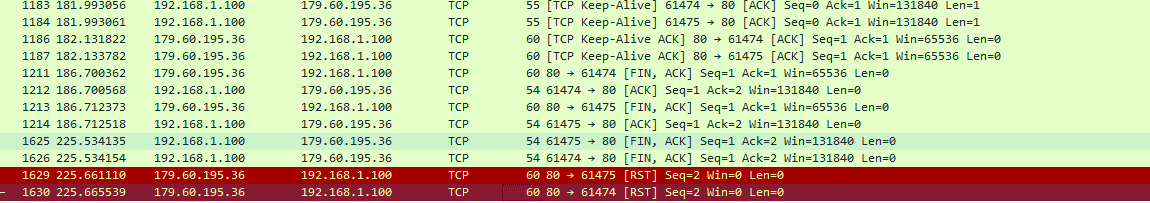
\includegraphics[width = 0.5 \textwidth]{images/8.png}
\end{center}

در ابتدا تعدادی بسته اولیه رد و بدل شده اما نتیجه نهایی به \lr{TCP RST} ختم شده است و همچنین با بررسی محتویات پیام‌های TCP آمده متوجه می‌شویم که همگی آن‌ها بسیار کوتاه هستند و اطلاعات کافی سایت را در بر ندارند.


\begin{center}
	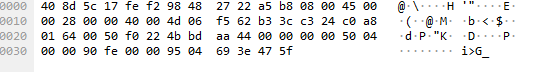
\includegraphics[width = 0.5 \textwidth]{images/9.png}
\end{center}

دلیل این موضوع هم این است که عملا فیلترینگ برای این سایت‌ها صرفا از لایه DNS نیست. بلکه به نوشته ویکی‌پدیا تکنولوژی \lr{Deep Packet Inspecting} در بخش فیلترینگ به کار رفته که جزئیات بسته‌های رد و بدل شده را بررسی می‌کند. بدین ترتیب مواردی نظیر آدرس مبدا یا مقصد و همچنین محتویات و کلمات استفاده شده در متن پیام در صورت رمزنگاری نشدن آن می‌تواند باعث بشود که Packet مورد نظر به عنوان محتوای فیلتر شده شناسایی شده و بعد از رسیدن به ISP ها Drop شود و در مواردی نظیر بالا تنها شامل رسیدن بسته‌هایی با متحوای بسیار کم هستیم. به علاوه به نظر می‌رسد که در مواردی تکنولوژی DPI حتی می‌تواند محتوای حدودی پیام‌های رمزنگاری شده و این که مربوط به چه مواردی هستند را هم تا حدی تشخیص بدهد و از این طریق هم امکان اعمال فیلترینگ وجود دارد.

علاوه بر این \textbf{نکته مهم} دیگری هم وجود دارد و آن هم بررسی بسته http ارسال شده است. با بررسی این بسته‌ها به مورد زیر می‌رسیم:

\begin{center}
	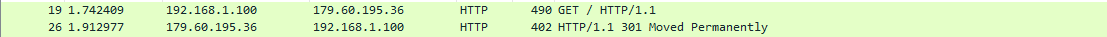
\includegraphics[width = 0.5 \textwidth]{images/10.png}
\end{center}

پاسخ دریافت شده برای درخواست \lr{\Verb+GET+} از این آدرس، کد \lr{\Verb+301 Moved Permanently+} است.


\begin{latin}
	\begin{verbatim}
	Hypertext Transfer Protocol
	HTTP/1.1 301 Moved Permanently\r\n
	Location: http://www.facebook.com/\r\n
	Content-Type: text/html; charset="utf-8"\r\n
	Date: Fri, 30 Apr 2021 15:11:44 GMT\r\n
	Alt-Svc: h3-29=":443"; ma=3600,h3-27=":443"; ma=3600\r\n
	Connection: keep-alive\r\n
	Content-Length: 0\r\n
	\r\n
	[HTTP response 1/1]
	[Time since request: 0.170568000 seconds]
	[Request in frame: 19]
	[Request URI: http://179.60.195.36/]
		
	\end{verbatim}
\end{latin}

آدرس جدید این سایت \lr{facebook.com} اعلام شده است. در نتیجه دوباره سیستم سعی‌ می‌کند از طریق DNS آدرس جدید را پیدا کند ولی در این زمینه هم با فیلترینگ مربوط به DNS رو به رو می‌شود و با آدرس \lr{\Verb+10.10.34.36+} رو‌به‌رو می‌شود که آدرس معتبری نیست.

	
\end{enumerate}

\section{سوال دوم}

\begin{enumerate}
	\item 
	پروتکل \lr{QUIC} یک پروتکل برای لایه انتقال است که توسط گوگل طراحی شده و  اکنون بعد از چندین سال طی مراحل آزمایشی، توسط \lr{IETF} به عنوان استاندارد جدید پذیرفته شده است. این پروتکل در مراحل اولیه توسط مروگر \lr{Chrome} و برای ارتباط با بعضی از سرویس‌ها و سایت‌های گوگل استفاده می‌شد اما اکنون شاهد گسترش استفاده آن و اضافه شدن پشتیبانی از آن به مرورگرهای دیگر هم اضافه شده است.
	
	هدف اصلی از طراحی \lr{QUIC}، ایجاد پروتکلی بوده است که هم به انتقال ترافیک \lr{HTTP} و \lr{HTTPS} سرعت بخشیده و هم امن‌تر باشد. این پروتکل بر پایه \lr{UDP} بنا شده است تا برای پیاده‌سازی آن نیاز به تغییر \lr{Middle-Box} های میانی ساختار شبکه نباشد. این پروتوکل سعی دارد با یکی کردن مراحل مربوط به \lr{Handshake} پروتکل‌های \lr{TCP} و همچنین پروتکل \lr{TLS} که برای \lr{HTTPS} استفاده می‌شود را در یک پروتکل یکپارچه کند و همچنین امکانات مربوط به \lr{Multiplexing} در \lr{HTTP/2} را هم به شکلی بهتر برای جلوگیری از \lr{HOL Blocking} پیاده‌سازی کند.
	
	\item
	
	در پروتکل \lr{HTTP/2} امکان \lr{Multiplexing} درخواست ها فراهم شد. به این شکل که به جای این که چندین \lr{Connection} از نوع \lr{TCP} برقرار شود که هر کدام اطلاعات بخشی از صفحه را دریافت کنند، یک اتصال \lr{TCP} ایجاد شده و بسته به این که هر قسمت متعلق به کدام بخش صفحه است، \lr{Multiplexing} صورت گرفته و به یکی از آن‌ها تعلق می‌گیرد.
	
	\begin{center}
		
		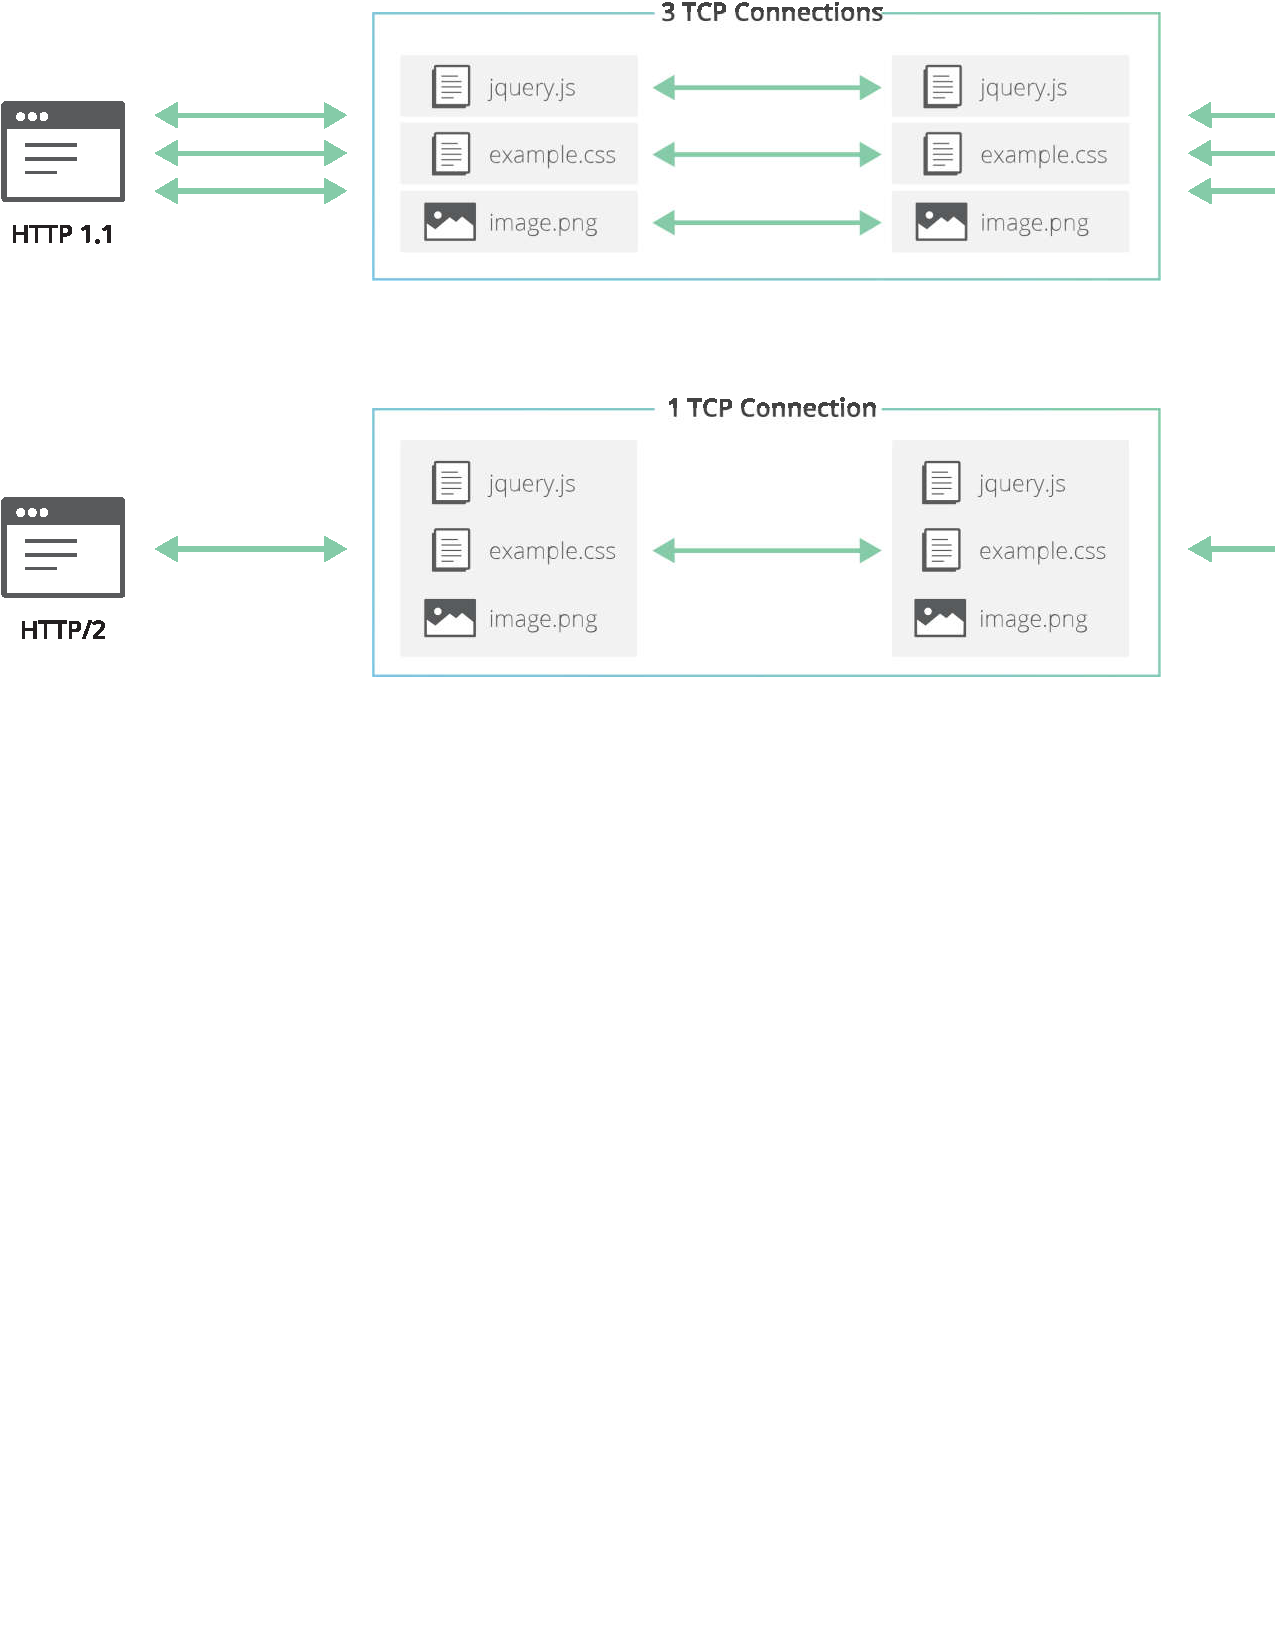
\includegraphics[width = 0.6\textwidth , trim=0 200 0 0]{images/multiplexing.pdf}
	\end{center}
	
	تنها ایرادی که در این زمینه وجود دارد مشکل \lr{Head of Line Blocking} است. در این حالت اگر یکی از پکت‌های \lr{TCP} از دست برود، باید منتظر ارسال مجدد آن بمانیم و عملا مزایای \lr{Multiplexing}‌ از بین می‌رود و با وجود تقسیم شدن به سگمنت‌های مختلف، همگی ‌آن‌ها معطل رسیدن بسته از دست رفته خواهند بود.
	
	با این حال \lr{QUIC} از پایه به این شکل طراحی شده است که \lr{Multiplexing} را به طور کامل پشتیبانی کند. این پروتکل قسمت‌های مختلف صفحه را به \lr{Stream} های مجزا تقسیم می‌:ند. از دست رفتن داده در یک پکت خاص مربوط به یک \lr{Stream} مشخص، تنها منجر به معطل شدن همان \lr{Stream} شده و بقیه \lr{Stream Frame} ها می‌توانند با موفقیت بعد از دریافت به بخش مربوطه متصل شده و معطل رسیدن بسته \lr{Stream} از دست رفته نخواهند بود. در این اتصال استریم‌های مختلف \lr{HTTP} می‌توانند به استریم‌های مختلف \lr{QUIC} مرتبط بشوند. ضمن این که همه این استریم‌ها از یک کانکشن \lr{QUIC} استفاده کرده و در نتیجه نیازی به انجام \lr{handshake}‌ های مجدد ندارند.


نتیجه نهایی همه این موارد این است که در اکثر اوقات، از دست رفتن یک پکت در یک استریم منجر به ایرادی یا بلاک شدن بقیه نمی‌شود و بقیه می‌توانند با موفقیت مراحل انتقال خود را انجام بدهند.


\item

اتصال \lr{QUIC} را کلاینت که یکی از \lr{Endpoint} های اتصال است برقرار می‌کند. در \lr{QUIC} اطلاعات مربوط به ورژن، رمزنگاری و \lr{Handshake} های اولیه همگی با هم صورت می‌گیرند تا تاخیری که در اثر مراحل شروع کار صورت می‌گیرد کاهش یابد. 

هر کدام از پکت‌های اولیه که توسط کلاینت ارسال می‌شوند باید فلگ مربوط به ورژن را به حالت \lr{On} در آورده و جزییات ورژن مورد استفاده را در میان بگذراند. تمامی پکت‌های ارسالی کلاینت در ابتدا این فلگ را در حالت \lr{On} می گذراند تا زمانی که یک جواب از سمت سرور با فلگ ورژن \lr{Off} دریافت شود. سرور هم پس از این که اولین پکتی از کلاینت را دریافت کرد که فلگ ورژن آن \lr{Off} بود، باید پکت‌های دیگری که با فلگ \lr{On} ممکن است به دلیل تاخیر دریافت شوند را نادیده بگیرد.

هنگامی که سرور یک پکت با \lr{Connection ID} جدیدی را دریافت می‌کند، ورژن آن را با ورژن‌هایی که پشتیبانی می‌کند مقایسه می‌:ند و اگر از آن پشتیبانی می‌کرد، تا انتهای عمر این اتصال از آن استفاده می‌کند.

در صورتی که این ورژن قابل قبول نباشد، با تاخیر یک \lr{Round-Trip Time} از سمت سرور یک پکت برای مذاکره در مورد ورژن به کلاینت ارسال می‌شود که در آن فلگ ورژن On بوده و لیست ورژن‌های قابل قبول در آن آمده است. کلاینت هم پس از دریافت این موضوع، یکی از آن آن پروتکل‌ّا را انتخاب کرده و براساس آن اطلاعات را از ابتدا باز ارسال می‌کند.

برای جلوگیری از حملات \lr{Donwgrading}، جزییات مربوط به ورژن که کلاینت در ابتدا مشخص کرده و ورژن‌های پشتیبانی شده توسط سرور در اطلاعات مربوط به \lr{Handshake} رمزنگاری هم قرار می‌گیرند تا کلاینت با چک کردن آن‌ها بتواند از صحت این اطلاعات اطمینان حاصل کند.

در همین مراحل اطلاعات مربوط به رمزنگاری و \lr{Handshake} اولیه لایه انتقال هم انجام می‌گیرد. یعنی همزمان مراحل انتقال جزییات رمزنگاری و \lr{Handshake} لازم با هم انجام می‌شود. \lr{QUIC} در ورژن‌های فعلی خود از پروتوکل \lr{TLS} برای رمزنگاری استفاده می‌کند اما این امکان وجود دارد که در آینده امکان استفاده از پروتکل‌های دیگری هم مهیا بشود. در حین انجام عملیات \lr{Handshake}، اطلاعات سطح \lr{Application} هم امکان انتقال دارند. به شکل ساده، ارتباط اولیه رمزنگاری به چنین شکلی قابل انجام است:

\begin{center}

\begin{latin}
	\begin{Verbatim}
	Client                                               Server
	
	Initial (CRYPTO)
	0-RTT (*)              ----------->
							Initial (CRYPTO)
							Handshake (CRYPTO)
				<----------                1-RTT (*)
	Handshake (CRYPTO)
	1-RTT (*)              ----------->
				<----------   1-RTT (HANDSHAKE_DONE)
	
	1-RTT                  <=========>                    1-RTT
	\end{Verbatim}
\end{latin}
	
\end{center}

	در همین مرحله، می‌توان اطلاعات مربوط به \lr{Explicit Congestion Notification} را هم منتقل کرد که مشخص کند آیا یکی از طرفین درگیر \lr{Congestion} شده است یا نه که طرف دیگر بداند باید با نرخ ارسال پایین اطلاعات را ارسال کند یا نه.
	
	
	در مورد اتمام اتصال، روش به این صورت است که اتصالات بعد از این که در وضعیت Idle‌ یا بلااستفاده قرار بگیرند، برای مدتی باز می‌ماند و پس از گذشت آن زمان، سرور اتصال را قطع می‌:ند. این قطع شدن اتصال لزوما با خبر کردن کلاینت همراه نخواهد بود چون اگر این اتصال در دستگاه‌های همراه (موبایل‌ها) برقرار شود، این کار نیازمندی فعال‌سازی دوباره اینترنت در این دستگاه‌ها بوده و منجر به مصرف برق می شود. در اصل به طور کلی دو نوع بسته شدن اتصال وجود دارد:
	
\begin{itemize}
	\item 
	خاموشی صریح: در این حالت یکی از \lr{Endpoint} ها یک فریم \lr{\Verb+CONNECTION\_CLOSE+} برای \lr{Endpoint}‌ دیگر ارسال می‌کند که آغازگر اتمام ارتباط است. \lr{Endpoint}‌دیگر می‌تواند یک فریم \lr{\Verb+GOAWAY+}‌ارسال کند که به معنی این است که به زودی ارتباط بسته خواهد شد. ارسال این سیگنال مشخص می‌کند که استریم‌های فعلی همچنان به کار خود اادامه می‌دهند تا به اتمام برسند ولی دیگر \lr{Stream} جدیدی ایجاد نخواهد شد تا بعد از اتمام کار قبلی‌ها، کار به اتمام برسد. بعد از اتمام کار دوباره \lr{\Verb+CONNECTION\_CLOSE+} ارسال می‌شود و اتصال به اتمام می‌رسد. اگر در حالی که هنوز استریم‌های ناتمام داریم این فریم ارسال شود، سمت دیگر باید این طور فرض کند که استریم‌ها به پایان نرسیده بودند ولی به شکل غیر منتظره بسته شدند.
	
	\item
	خاموشی ضمنی: تایم‌اوت پیش‌فرض برای قرار گرفتن یک اتصال در وضعیت بلااستفاده $30$ ثانیه است و در همان ابتدای ایجاد به عنوان یک پارامتر ضروری که \lr{\Verb+ICSL+} نام دارد باید مشخص بشود. حداکثر زمانی هم که می‌توان برای این کار تعیین کرد $10$ دقیقه است. اگر هیچ فعالیتی روی این اتصال به اندازه زمان مشخص شده وجود نداشته باشد، اتصال بسته می‌شود. در هنگام بسته شدن، به طور پیش‌فرض یک فریم \lr{\Verb+CONNECTION\_CLOSE+} ارسال می‌شود ولی می‌توان ارسال آن را غیرفعال کرد تا در شبکه‌هایی که هزینه ارسال بالاست (نظیر شبکه‌های موبایل)، بدون دریافت پیام جدید در سمت دیگر، اتصال بسته بشود.
	
	
\end{itemize}

در زیر دو مقایسه بین اتصال \lr{TCP} رایج به همراه رمزنگاری \lr{TLS} که برای شروع نیاز به دو \lr{RTT} دارد با پروتکل \lr{QUIC} که با یک \lr{RTT} این کار را انجام می‌دهد قرار گرفته است:


\begin{center}
	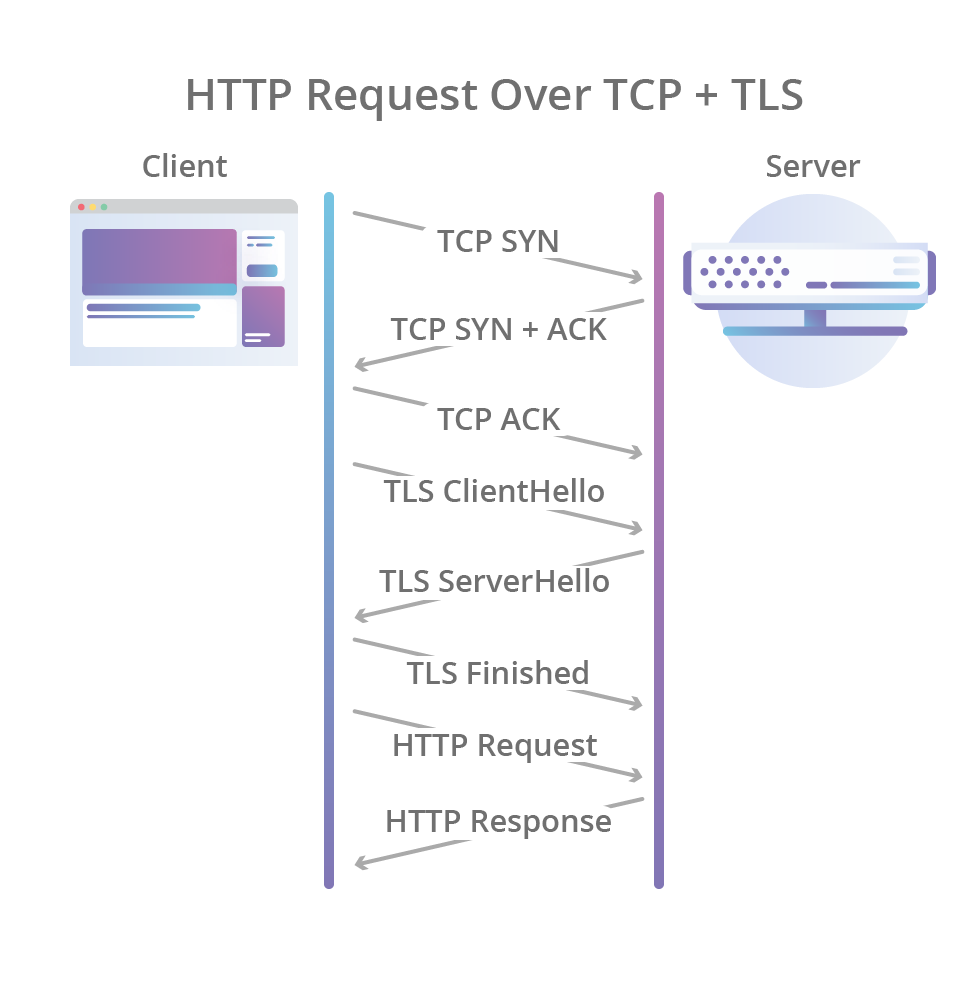
\includegraphics[width = 0.55 \textwidth]{images/11.png}
\end{center}


\begin{center}
	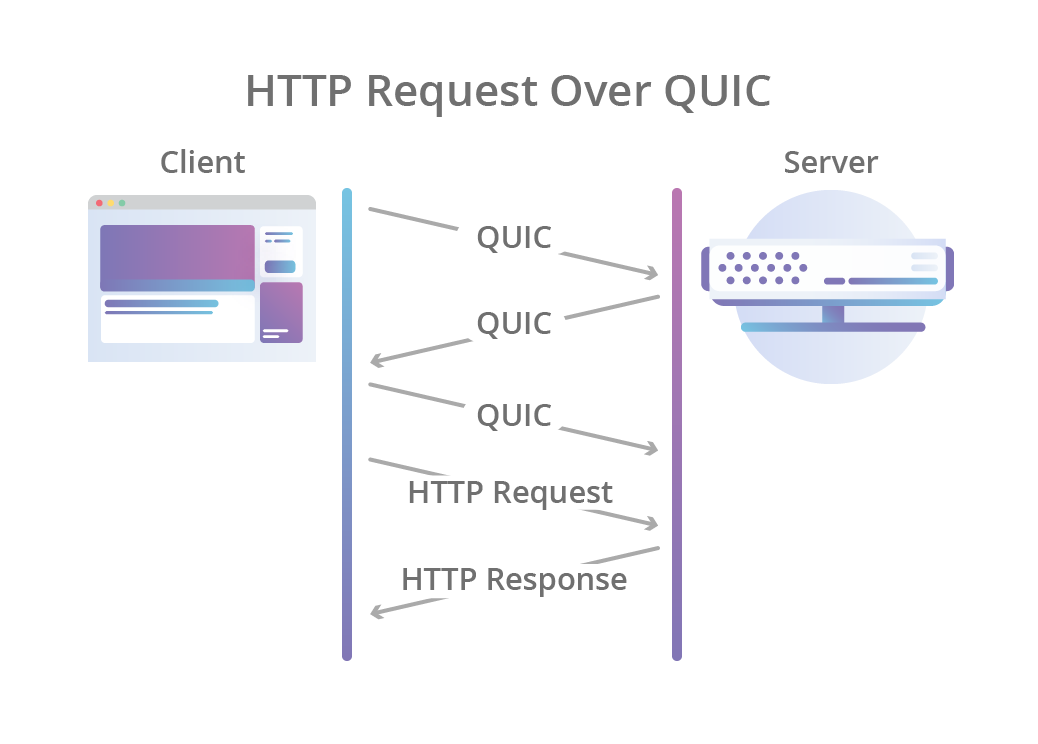
\includegraphics[width = 0.55 \textwidth]{images/12.png}
\end{center}


\item

این قسمت براساس درفت هشتم \lr{QUIC} نوشته شده است (لینک داده شده در صورت سوال درفت دوم \lr{QUIC} است):

\begin{latin}
\textcolor{Blue}{{\underline{\textcolor{Blue}{ \href{https://tools.ietf.org/html/draft-ietf-quic-transport-08}{https://tools.ietf.org/html/draft-ietf-quic-transport-08}}}}}
\end{latin}

ابتدا باید توجه کنیم که همه داده‌های عددی به صورت Big-Endian انکود شده و ارسال می‌شوند. در نتیجه با ارزش‌ترین بیت، بیت صفرم است.

هر بسته کوئیک می‌تواند هدر بلند یا هدر کوتاه داشته باشد. هدر‌های بلند ممولا برای مشخص کردن ورژن اولیه و شروع اتصال استفاده می‌شوند. پس از آن از هدرهای کوتاه استفاده می‌شود.


هدر بلند ساختاری مانند زیر دارد:


	\begin{center}
\begin{latin}

	\begin{Verbatim}
0                   1                   2                   3
0 1 2 3 4 5 6 7 8 9 0 1 2 3 4 5 6 7 8 9 0 1 2 3 4 5 6 7 8 9 0 1
+-+-+-+-+-+-+-+-+
|1|   Type (7)  |
+-+-+-+-+-+-+-+-+-+-+-+-+-+-+-+-+-+-+-+-+-+-+-+-+-+-+-+-+-+-+-+-+
|                                                               |
+                       Connection ID (64)                      +
|                                                               |
+-+-+-+-+-+-+-+-+-+-+-+-+-+-+-+-+-+-+-+-+-+-+-+-+-+-+-+-+-+-+-+-+
|                         Version (32)                          |
+-+-+-+-+-+-+-+-+-+-+-+-+-+-+-+-+-+-+-+-+-+-+-+-+-+-+-+-+-+-+-+-+
|                       Packet Number (32)                      |
+-+-+-+-+-+-+-+-+-+-+-+-+-+-+-+-+-+-+-+-+-+-+-+-+-+-+-+-+-+-+-+-+
|                          Payload (*)                        ...
+-+-+-+-+-+-+-+-+-+-+-+-+-+-+-+-+-+-+-+-+-+-+-+-+-+-+-+-+-+-+-+-+

	\end{Verbatim}
	

\end{latin}
\end{center}

این هدرها قبل از کامل شدن فرآیند ارتباط اولیه و مشخص شدن ورژن استفاده می‌شوند.

 بیت اول بسته $1$ است. هفت بیت بعدی بیانگر نوع بسته هستند و $128$ نوع بسته مختلف می‌تواند برای این فیلد در نظر گرفته بشود اما فعلا از همه‌ آن‌ها استفاده نمی‌شود.  بعد از آن $64$ بیت برای مشخص کردن \lr{Connection ID} می‌آیند که عملا عامل تمایز اصلی بین اتصالات است.
پس از آن $32$ برای مشخص کردن ورژن \lr{QUIC} استفاد هشده و مشخص می‌کند که سایر هدر‌ها و فیلدهای پیام به چه شکل تفسیر می‌شوند. پس آز آن هم \lr{Packet Number} می‌آید که $32$ بیتی است اما می‌تواند بیانگر عددی بین $0$ تا $2^{62}-1$ باشد اما به شیوه خاصی تنها $32$ کم ارزش‌ آن ارسال می‌شوند. بعد از این‌ها بخش اصلی و \lr{Payload} پیام قرار می‌گیرد.

انواع پکت‌هایی که با حالت Long ارسال می‌شوند شامل چهار پکت هستند.

\begin{latin}
\begin{itemize}
	\item \lr{\Verb+0x7F:		Initial+}
	
	\item \lr{\Verb+0x7E:		Retry+}
	
	
	\item \lr{\Verb+0x7D:		Handshake+}
	
	
	\item \lr{\Verb+0x7C:		0-RTT Protected+}
\end{itemize}
\end{latin}

نحوه تفسیر \lr{Payload} و فیلد‌های خاص درون آن بسته به ورژن‌های مختلف \lr{QUIC} می‌تواند متفاوت باشد.
	
	
	هدر کوتاه ساختاری مانند زیر دارد:
	
	\begin{latin}
		\begin{center}
			\begin{Verbatim}
0                   1                   2                   3
0 1 2 3 4 5 6 7 8 9 0 1 2 3 4 5 6 7 8 9 0 1 2 3 4 5 6 7 8 9 0 1
+-+-+-+-+-+-+-+-+
|0|C|K| Type (5)|
+-+-+-+-+-+-+-+-+-+-+-+-+-+-+-+-+-+-+-+-+-+-+-+-+-+-+-+-+-+-+-+-+
|                                                               |
+                     [Connection ID (64)]                      +
|                                                               |
+-+-+-+-+-+-+-+-+-+-+-+-+-+-+-+-+-+-+-+-+-+-+-+-+-+-+-+-+-+-+-+-+
|                      Packet Number (8/16/32)                ...
+-+-+-+-+-+-+-+-+-+-+-+-+-+-+-+-+-+-+-+-+-+-+-+-+-+-+-+-+-+-+-+-+
|                     Protected Payload (*)                   ...
+-+-+-+-+-+-+-+-+-+-+-+-+-+-+-+-+-+-+-+-+-+-+-+-+-+-+-+-+-+-+-+-+

			\end{Verbatim}
			
		\end{center}
	\end{latin}
	
	


اولین بیت در این نوع هدر برابر $0$ است. بیت دوم اصطلاحا بیت \lr{Omit Connection ID Flag} است و در صورتی که $0$ باشد \lr{Connection ID} را در ادامه هدر خواهیم داشت و در غیر این صورت، \lr{Connection ID} را نخواهیم داشت. بیت بعدی \lr{Key Phase Bit} است که به شناسایی کلید‌های حفاظتی که در پکت قرار دارند در سمت گیرنده کمک می‌کند. جزییات دقیق این موضوع به نحوه پیاده‌سازی سیستم رمزنگاری \lr{QUIC-TLS} ربط دارد و خارج از مقوله این سوال است.

پس از این $5$ بیت برای تعیین نوع بسته وجود دارد. بسته‌های کوتاه می‌توانند $32$ نوع مختلف داشته باشند اما فعلا از همه این $32$ نوع استفاده نشده است.

پس از آن $64$ بیت \lr{Connection ID} می‌تواند وجود داشته باشد. در صورتی که فیلد \lr{Omit Connection ID Flag} برابر $1$ باشد این قسمت را نخواهیم داشت.

پس از آن شماره بسته (\ lr{Packet Number}) می‌آید. بسته به نوع بسته این شماره می‌تواند $8$، $16$ یا $32$ بیتی باشد. پس از آن هم قسمت \lr{Protected Payload} قرار دارد.

براساس پیاده‌سازی‌ها، انواع پکت‌های کوتاه فعلا شامل سه نوع (از $32$ نوع ممکن) است که طول \lr{Packet Number} را مشخص می‌کند.


\begin{latin}
	\begin{itemize}
		\item \lr{\Verb+0x1F:		8-bit Packet Number+}
		
		\item \lr{\Verb+0x1E:		16-bit Packet Number+}
		
		
		\item \lr{\Verb+0x1D:		32-bit Packet Number+}
		
		
	
	\end{itemize}
\end{latin}

با تمام این‌ها به نظر تغییراتی در این فرمتینگ در نسخه‌‌های جدید‌تر \lr{QUIC} داده شده است و خصوصا در حالت \lr{Short} شاهد اضافه شدن یکسری فلگ‌های تک‌بیتی دیگر هم هستیم.


\item
برای این مورد ابتدا باید به نحوه ارسال پکت‌ها در \lr{QUIC} توجه کنیم. در ارسال بسته‌ها، هر بسته شامل \lr{Packet Number}‌است. این شماره بسته در طول عمر یک اتصال هیچ‌وقت تکرار نشده و مقدار آن‌هم به شکل اکیدا صعودی افزایش می‌یابد. در نتیجه شناسایی مواردی که دو بار ارسال شده اند به راحتی امکان پذیر است.

هر بسته می‌تواند شامل چندین فریم باشد. دو فریم اصلی که برای ما اهمیت دارند، یکی فریم \lr{STREAM} است که دیتای اصلی را در خود دارد و البته اطلاعات مربوط به \lr{Handshake}‌ رمزنگاری هم در آن قرار می‌گیرند. بخش دیگر فریم‌های \lr{ACK} هستند. \lr{QUIC}‌ از سیستم \lr{NACK} یا \lr{Negative Acknowledgment} استفاده می‌‌کند. بدین شکل که بیش‌ترین شماره پکتی که دیده شده ارسال شده و در کنار آن، شماره پکت‌هایی که کمتر از آن هستند و دریافت نشده‌اند به عنوان بازه‌های NACK‌ارسال می‌شوند تا آن موارد باز ارسال بشوند. همچنین در فریم مربوط به \lr{ACK} یک \lr{timestamp} برای مشخص کردن زمان ارسال این پیام هم قرار دارد. همچنین \lr{QUIC} امکان استفاده از $255$ بازه \lr{NACK} را دارد که در محیط‌هایی که امکان \lr{Loss}‌ بالاست، باعث سرعت بخشیدن به بازیابی می‌شود. همچنین مشخص کردن زمان \lr{ACK} باعث می‌شود که گیرنده \lr{ACK} متوجه اختلاف زمانی بین ارسال \lr{ACK} و دریافت بسته اصلی بشود و ارسال بسته‌های بعدی را متناسب با آن تنظیم کند. (مثلا بررسی کند که یکسری از بسته‌ها که \lr{ACK} آن‌ها دریافت نشده، احتمالا در زمان فعلی به دست گیرنده رسیده و صرفا هنوز \lr{ACK} آن‌ها نرسیده است، در نتیجه فرآیند را از بسته‌های بعدی ادامه بدهد)

با توجه به این مقدمه مکانیزم \lr{Loss Recovery} در \lr{QUIC} به این شکل است:

\begin{itemize}
	\item در هنگام ارسال بسته:
	
	\begin{itemize}
		\item اگر \lr{Handshake} به درستی صورت نگرفته باشد، یک تایمر استارت زده شده و مقدار اولیه آن $1.5$ برابر \lr{SRTT} بوده و کاهش نرخ ارسال آن به صورت نمایی است.
		
		\item
		
		اگر تعداد زیادی بسته \lr{NACK} شده اند، احتمالا باید \lr{timer} مربوط به از دست رفتن را استارت زد. مقدار پیش‌فرض آن $0.25 RTT$ است.
		
		\item
		
		اگر کمتر از $2$ پکت لایه انتقال ارسال شده است، تایمر مربوط ه ریستار می‌شود. اگر چندین پکت در راه ارسال باشند، مقدار آن برابر ماکسیمم $10ms$ و $2 \times SRTF$ خواهد بود و اگر تنها تنها یک بسته در راه باشد مقدار آن برابر
		$\max(1.5\times SRTF + \text{delayed ack timer} + 2\times SRTF)$
		خواهد بود.
		
		\item
		
		اگر حداقل دو بسته لایه انتقال ارسال شده است، تایمر \lr{Retransmission Timeout} را استارت می‌زنیم و مقدار آن برابر
		$\max(200ms , SRTT + 4 \times RTTVAR)$
		خواهد بود و بعد از اولین تایم‌اوت مجدد، مقدار آن به صورت نمایی کم خواهد شد.
	\end{itemize}


\item در هنگام دریافت \lr{ACK}:

در هنگام دریافت \lr{ACK} مراحل زیر طی می‌شود:
\begin{itemize}
	\item 
	این \lr{ACK} صحت سنجی و اعتبارسنجی شده و \lr{ACK} هایی که بدون ترتیب آمده ‌اند و یا قبلا \lr{ACK} آن‌ها دریافت شده نادیده گرفته می شوند.
	
	\item
	مقادیر مربوط به \lr{RTT} دوباره محاسبه شده و آپدیت می‌شوند.
	
	\item
	ارسال کننده که \lr{ACK} را دریافت کرده، بسته‌هایی که مقدارشان از \lr{Packent Number} این \lr{ACK} کمتر بوده و جزو بخش \lr{NACK} نیستند را به عنوان موارد \lr{ACKED} شده علامت گذاری می‌کند.
	
	\item
	بسته‌هایی که مقدار \lr{Packet Number} آن‌ها کمتر از بیش‌تری \lr{ACK} مشاهده شده بوده و در دسته \lr{NACK} ها باشند، به عنوان بسته‌های گمشده علامت گذاری می‌شوند.
	
	\item
	حد آستانه‌ برای بسته‌های گمشده به طور پیش‌فرض برابر $3$ است.
	
	\item
	بسته‌هایی که بیش‌تر حد آستانه گفته شده گزارش گمشدن داشته باشند، برای ارسال مجدد آماده می‌شوند.
	
	\item
	اگر تعداد بسته‌های  \lr{NACK} شده زیاد باشند و مقدار بیش‌ترین بسته دیده‌شده برابر بزرگترین بسته ارسال شده باشد، تایمر ارسال مجدد برابر $0.25RTT$ می‌شود.
	
	\item
	در صورتی که بسته‌های \lr{NACK} شده خیلی قابل توجه نیستند، تایمر بخش قبل متوقف می‌شود.
	
\end{itemize}

\item هنگام به پایان رسیدن تایمر:

پروتکل \lr{QUIC} از یک تایمر \lr{Loss Recovery} استفاده می‌کند که هنگام ست شدن، می تواند در حالت‌های مختلفی باشد. این وضعیت عملی که باید انجام شود را مشخص می‌کند.

\begin{itemize}
	\item در حالت \lr{Handshake}
	\begin{itemize}
		\item بسته‌های \lr{Handshake} دوباره ارسال می‌شوند.
	\end{itemize}

\item در حالت \lr{Loss}

\begin{itemize}
	\item بسته‌های قابل توجهی که \lr{NACK} شده‌اند به عنوان از دست رفته شده در نظر گرفته می شوند.
	
	\item این از دست رفتن به کنترلر بخش \lr{Congestion} گزارش می شود.
	
	\item بسته به میزانی که کنترلر \lr{Congestion} اجازه بدهد، بسته‌ها بازارسال می‌شوند.
	\end{itemize}

\item در حالت \lr{TLP} (بسته لایه انتقال)

\begin{itemize}
	\item کوچک‌‌ترین بسته‌ای که به میزان قابل توجهی \lr{LOSS} شده است و قابل ارسال مجدد است را ارسال می‌کنیم.
	
	\item هیچ بسته‌ای را به عنوان گمشده علامت‌گذاری نمی‌کنیم تا \lr{ACK} بعدی برسد.
	
	\item
	تایمر را برای حالت \lr{TLP} یا \lr{RTO} ریستارت می‌کنیم.
\end{itemize}

\item حالت \lr{RTO}:
کلمه \lr{RTO} به معنی \lr{Retransmission Timeout} است.

\begin{itemize}
	\item دو بسته‌ای که به میزان قابل توجهی \lr{Loss} برای آنان گزارش شده و سایز کمتری داشته و قابل ارسال مجدد هستند، دوباره ارسال می‌شود.
	
	\item
	
	مقدار \lr{Congestion Window} برابر $1$ بسته شده و منتظر می‌مانیم تا \lr{Ack} بعدی برسد تا مطمئن شویم که \lr{RTO} ما اضافی نبوده است.
	
	\item
	تایمر برای \lr{RTO} بعدی ریست می‌شود. (با نرخ \lr{Backoff} نمایی)
\end{itemize}
\end{itemize}
\end{itemize}

\end{enumerate}

\newpage
\section{سوال سوم}

تمامی موارد با اتصال به کنترلر \lr{Floodlight} اجرا شده‌اند.

\begin{enumerate}
	\item 
	بعد از اجرای اسکریپت پایتون، دستورات زیر را اجرا می‌کنیم:
	
	\begin{latin}
	\begin{lstlisting}[language=bash]
		xterm h1 h3
	\end{lstlisting}
\end{latin}

با \lr{\Verb+ifconfig+} متوجه‌ می‌شویم که IP هاست اول \lr{\Verb+10.0.0.1+} است.

دستور زیر را در هاست اول اجرا می‌کنیم:
	
\begin{latin}
	\begin{lstlisting}[language=bash]
		iperf3 -s
	\end{lstlisting}
\end{latin}

و در هاست سوم دستور زیر را اجرا می‌کنیم:
\begin{latin}
	\begin{lstlisting}[language=bash]
		iperf3 -c 10.0.0.1 -t 10
	\end{lstlisting}
\end{latin}

\begin{latin}
	\begin{Verbatim}
Connecting to host 10.0.0.1, port 5201
[  6] local 10.0.0.3 port 47408 connected to 10.0.0.1 port 5201
[ ID] Interval           Transfer     Bandwidth       Retr  Cwnd
[  6]   0.00-1.00   sec  2.42 MBytes  20.3 Mbits/sec    0   31.1 KBytes       
[  6]   1.00-2.00   sec  2.24 MBytes  18.8 Mbits/sec    0   31.1 KBytes       
[  6]   2.00-3.00   sec  2.24 MBytes  18.8 Mbits/sec    0   31.1 KBytes       
[  6]   3.00-4.00   sec  2.24 MBytes  18.7 Mbits/sec    0   31.1 KBytes       
[  6]   4.00-5.00   sec  2.24 MBytes  18.8 Mbits/sec    0   31.1 KBytes       
[  6]   5.00-6.00   sec  2.17 MBytes  18.2 Mbits/sec    0   31.1 KBytes       
[  6]   6.00-7.00   sec  2.30 MBytes  19.3 Mbits/sec    0   31.1 KBytes       
[  6]   7.00-8.00   sec  2.11 MBytes  17.7 Mbits/sec    0   31.1 KBytes       
[  6]   8.00-9.00   sec  2.30 MBytes  19.3 Mbits/sec    0   31.1 KBytes       
[  6]   9.00-10.00  sec  2.17 MBytes  18.3 Mbits/sec    0   31.1 KBytes       
- - - - - - - - - - - - - - - - - - - - - - - - -
[ ID] Interval           Transfer     Bandwidth       Retr
[  6]   0.00-10.00  sec  22.4 MBytes  18.8 Mbits/sec    0             sender
[  6]   0.00-10.00  sec  22.3 MBytes  18.7 Mbits/sec                  receiver
	
		
	\end{Verbatim}
\end{latin}

همان طور که مشاهده‌ می‌شود، گذردهی نهایی \lr{\Verb+18.8 Mbits/sec+} گزارش شده است. چیزی که انتظار داریم در اصل $20$ است اما این عدد هم تفاوت چندانی ندارد.  دلیل این تفاوت می‌تواند به این مربوط باشد که در این جا عملا یک سوییچ واقعی شبیه سازی شده است و یکسری پارامترهای درونی خود پروتکل \lr{OpenFlow1.3} و همچنین کنترلر \lr{Floodlight} تاثیرگذار بوده‌اند. مخصوصا در قسمت‌های بعدی شاهد تفاوت‌های جدی‌تری خواهیم بود که آن ها را بهتر می‌توان توجیه کرد. 

ضمنا اعداد بالا تا حد خوبی برای هر دو طرف یکسان هستند و تفاوت معناداری بین‌‌ آن‌ها مشاهده نمی‌شود.

\item
دستورات مشابهی را مانند بالا برای هاست اول و دوم اجرا می‌کنیم.

نتایج برای هر کدام از طرفین متفاوت است. برای فرستنده:


\begin{latin}
	\begin{Verbatim}
[  6] local 10.0.0.2 port 43558 connected to 10.0.0.1 port 5201
[ ID] Interval           Transfer     Bandwidth       Retr  Cwnd
[  6]   0.00-1.00   sec   362 KBytes  2.96 Mbits/sec    0    110 KBytes       
[  6]   1.00-2.00   sec  7.36 MBytes  61.7 Mbits/sec    0   1.38 MBytes       
[  6]   2.00-3.00   sec  3.75 MBytes  31.5 Mbits/sec    0   1.91 MBytes       
[  6]   3.00-4.00   sec  2.50 MBytes  21.0 Mbits/sec    0   2.02 MBytes       
[  6]   4.00-5.00   sec  2.50 MBytes  21.0 Mbits/sec    0   2.14 MBytes       
[  6]   5.00-6.00   sec  2.50 MBytes  21.0 Mbits/sec    0   2.25 MBytes       
[  6]   6.00-7.00   sec  2.50 MBytes  21.0 Mbits/sec    0   2.36 MBytes       
[  6]   7.00-8.00   sec  2.50 MBytes  21.0 Mbits/sec    0   2.48 MBytes       
[  6]   8.00-9.00   sec  2.50 MBytes  21.0 Mbits/sec    0   2.58 MBytes       
[  6]   9.00-10.00  sec  2.50 MBytes  21.0 Mbits/sec    0   2.69 MBytes       
- - - - - - - - - - - - - - - - - - - - - - - - -
[ ID] Interval           Transfer     Bandwidth       Retr
[  6]   0.00-10.00  sec  29.0 MBytes  24.3 Mbits/sec    0             sender
[  6]   0.00-10.00  sec  21.9 MBytes  18.4 Mbits/sec                 receiver
		
		
		
		
	\end{Verbatim}
\end{latin}

اما در سمت گیرنده شاهد چنین اعداد هستیم:

\begin{latin}
	\begin{Verbatim}
[  7] local 10.0.0.1 port 5201 connected to 10.0.0.2 port 43558
[ ID] Interval           Transfer     Bandwidth
[  7]   0.00-1.00   sec  82.0 KBytes   672 Kbits/sec                  
[  7]   1.00-2.00   sec  1.27 MBytes  10.7 Mbits/sec                  
[  7]   2.00-3.00   sec  2.27 MBytes  19.0 Mbits/sec                  
[  7]   3.00-4.00   sec  2.27 MBytes  19.0 Mbits/sec                  
[  7]   4.00-5.00   sec  2.27 MBytes  19.0 Mbits/sec                  
[  7]   5.00-6.00   sec  2.27 MBytes  19.0 Mbits/sec                  
[  7]   6.00-7.00   sec  2.27 MBytes  19.1 Mbits/sec                  
[  7]   7.00-8.00   sec  2.27 MBytes  19.0 Mbits/sec                  
[  7]   8.00-9.00   sec  1.97 MBytes  16.5 Mbits/sec                  
[  7]   9.00-10.00  sec  2.27 MBytes  19.0 Mbits/sec                  
[  7]  10.00-11.03  sec   662 KBytes  5.27 Mbits/sec                  
[  7]  11.03-12.37  sec  38.2 KBytes   233 Kbits/sec                  
[  7]  12.37-13.37  sec  80.6 KBytes   658 Kbits/sec                  
[  7]  13.37-14.37  sec   628 KBytes  5.18 Mbits/sec                  
[  7]  14.37-15.37  sec  17.0 KBytes   139 Kbits/sec                  
[  7]  15.37-16.37  sec  17.0 KBytes   138 Kbits/sec                  
[  7]  16.37-17.04  sec   105 KBytes  1.28 Mbits/sec                  
[  7]  17.04-18.03  sec   116 KBytes   963 Kbits/sec                  
[  7]  18.03-19.36  sec  46.7 KBytes   287 Kbits/sec                  
[  7]  19.36-20.36  sec  11.3 KBytes  92.7 Kbits/sec                  
[  7]  20.36-21.22  sec  91.9 KBytes   882 Kbits/sec                  
[  7]  21.22-22.36  sec  74.9 KBytes   537 Kbits/sec                  
[  7]  22.36-23.36  sec  18.4 KBytes   151 Kbits/sec                  
[  7]  23.36-24.36  sec   109 KBytes   891 Kbits/sec                  
[  7]  24.36-25.36  sec  15.6 KBytes   128 Kbits/sec                  
[  7]  25.36-26.36  sec  60.8 KBytes   499 Kbits/sec                  
[  7]  26.36-26.82  sec   679 KBytes  12.0 Mbits/sec                  
- - - - - - - - - - - - - - - - - - - - - - - - -
[ ID] Interval           Transfer     Bandwidth       Retr
[  7]   0.00-26.82  sec  29.0 MBytes  9.06 Mbits/sec    0             sender
[  7]   0.00-26.82  sec  21.9 MBytes  6.85 Mbits/sec                  receiver

	\end{Verbatim}
\end{latin}

مشاهده می‌کنیم که در سمت دریافت کننده اعداد \lr{Throughput} بسیار کمتر هستند. دلیل این موضوع به دلیل \lr{Latency} موجود در شبکه است. این موضوع باعث شده که بسته ها دیرتر به مقصد برسند و به علاوه شاهد تغییرات جدی در \lr{Congestion Window} سمت فرستنده هم هستیم.

اثر اصلی \lr{Latency} در این است که باعث می‌شود که Ack ها به موقع دریافت نشوند.

در حالت قبلی RTT کمتر از $1ms$ بود و تنها موضوعی که گلوگاه بود، سرعت خود لینک بود ولی در این جا RTT حدود $200ms$ است و این موضوع گلوگاه ایجاد کرده است.

\item


با اجرای دستورات مشابه، نتیجه زیر را داریم:

\begin{latin}
	\begin{Verbatim}

[  6] local 10.0.0.5 port 47704 connected to 10.0.0.4 port 5201
[ ID] Interval           Transfer     Bandwidth       Retr  Cwnd
[  6]   0.00-1.00   sec  2.16 MBytes  18.0 Mbits/sec   22   11.3 KBytes       
[  6]   1.00-2.00   sec  1.12 MBytes  9.36 Mbits/sec   12   9.90 KBytes       
[  6]   2.00-3.00   sec  1018 KBytes  8.38 Mbits/sec    4   11.3 KBytes       
[  6]   3.00-4.00   sec   891 KBytes  7.30 Mbits/sec    4   9.90 KBytes       
[  6]   4.00-5.00   sec  1018 KBytes  8.34 Mbits/sec    2   12.7 KBytes       
[  6]   5.00-6.00   sec   891 KBytes  7.29 Mbits/sec   12   9.90 KBytes       
[  6]   6.00-7.00   sec   764 KBytes  6.26 Mbits/sec    3   11.3 KBytes       
[  6]   7.00-8.00   sec  1018 KBytes  8.33 Mbits/sec    5   9.90 KBytes       
[  6]   8.00-9.00   sec  1.99 MBytes  16.7 Mbits/sec   18   14.1 KBytes       
[  6]   9.00-10.00  sec  2.24 MBytes  18.8 Mbits/sec   13   17.0 KBytes       
- - - - - - - - - - - - - - - - - - - - - - - - -
[ ID] Interval           Transfer     Bandwidth       Retr
[  6]   0.00-10.00  sec  13.0 MBytes  10.9 Mbits/sec   95             sender
[  6]   0.00-10.00  sec  12.8 MBytes  10.7 Mbits/sec                  receiver


	\end{Verbatim}
\end{latin}


برای سمت دیگر هم به همین شکل است. مشاهده‌ می‌کنیم که گذردهی و Bandwidth حدودا نصف شده است. 
در اصل Loss به دو شکل تاثیر گذار است. از یک سو نیاز به ارسال مجدد بسته‌های از دست رفته داریم. از سوی دیگر Cwnd نمی‌تواند به حالت بهینه ثابتی دست یابد. به علاوه تاثیر مستقیم آن‌هم این است که دیتایی که از دست رفته باشد را عملا نمی‌توان در Throughput به حساب آورد و همین موضوع هم موجب کاهش گذردهی می‌شود.


\item

سه رقم آخر $212$ است.

هاست چهارم را سرور می‌کنیم.

\begin{latin}
	\begin{lstlisting}[language=bash]
		iperf3 -s
	\end{lstlisting}
\end{latin}

و از هاست اول به آن داده ارسال می‌کنیم.

$$212 MB = 222298112 Byte$$


\begin{latin}
	\begin{lstlisting}[language=bash]
		 iperf3 -c 10.0.0.4 -J>result.json -n 222298112 
	\end{lstlisting}
\end{latin}

خروجی نهایی برای سمت گیرنده بدین شکل است:

\begin{latin}
\begin{Verbatim}
[  7] local 10.0.0.4 port 5201 connected to 10.0.0.1 port 39646
[ ID] Interval           Transfer     Bitrate
[  7]   0.00-1.00   sec  2.10 MBytes  17.6 Mbits/sec                  
[  7]   1.00-2.00   sec  2.25 MBytes  18.9 Mbits/sec                  
[  7]   2.00-3.00   sec  2.24 MBytes  18.8 Mbits/sec                  
[  7]   3.00-4.00   sec  2.25 MBytes  18.9 Mbits/sec                  
[  7]   4.00-5.00   sec  2.26 MBytes  18.9 Mbits/sec                  
[  7]   5.00-6.00   sec  2.26 MBytes  18.9 Mbits/sec                  
[  7]   6.00-7.00   sec  2.25 MBytes  18.9 Mbits/sec                  
[  7]   7.00-8.00   sec  2.25 MBytes  18.8 Mbits/sec                  
[  7]   8.00-9.00   sec  2.25 MBytes  18.8 Mbits/sec                  
[  7]   9.00-10.00  sec  2.24 MBytes  18.8 Mbits/sec                  
[  7]  10.00-11.00  sec  2.25 MBytes  18.8 Mbits/sec                  
[  7]  11.00-12.00  sec  2.25 MBytes  18.9 Mbits/sec                  
[  7]  12.00-13.00  sec  2.24 MBytes  18.8 Mbits/sec                  
[  7]  13.00-14.00  sec  2.23 MBytes  18.7 Mbits/sec                  
[  7]  14.00-15.00  sec  2.24 MBytes  18.8 Mbits/sec                  
[  7]  15.00-16.00  sec  2.25 MBytes  18.9 Mbits/sec                  
[  7]  16.00-17.00  sec  2.23 MBytes  18.7 Mbits/sec                  
[  7]  17.00-18.00  sec  2.25 MBytes  18.9 Mbits/sec                  
[  7]  18.00-19.00  sec  2.25 MBytes  18.9 Mbits/sec                  
[  7]  19.00-20.00  sec  93.3 KBytes   764 Kbits/sec                  
[  7]  20.00-21.00  sec  67.9 KBytes   556 Kbits/sec                  
[  7]  21.00-22.00  sec  5.41 MBytes  45.4 Mbits/sec                  
[  7]  22.00-23.00  sec   946 KBytes  7.74 Mbits/sec                  
[  7]  23.00-24.00  sec  1.35 MBytes  11.3 Mbits/sec                  
[  7]  24.00-25.00  sec  2.26 MBytes  18.9 Mbits/sec                  
[  7]  25.00-26.00  sec  2.26 MBytes  18.9 Mbits/sec                  
[  7]  26.00-27.00  sec  2.26 MBytes  18.9 Mbits/sec                  
[  7]  27.00-28.00  sec  2.26 MBytes  18.9 Mbits/sec                  
[  7]  28.00-29.00  sec  2.25 MBytes  18.9 Mbits/sec                  
[  7]  29.00-30.01  sec   949 KBytes  7.73 Mbits/sec                  
[  7]  30.01-31.00  sec   567 KBytes  4.67 Mbits/sec                  
[  7]  31.00-32.00  sec  1.48 MBytes  12.4 Mbits/sec                  
[  7]  32.00-33.00  sec  1.33 MBytes  11.2 Mbits/sec                  
[  7]  33.00-34.00  sec  1.46 MBytes  12.2 Mbits/sec                  
[  7]  34.00-35.00  sec  2.24 MBytes  18.8 Mbits/sec                  
[  7]  35.00-36.00  sec  1.69 MBytes  14.2 Mbits/sec                  
[  7]  36.00-37.00  sec  1.93 MBytes  16.2 Mbits/sec                  
[  7]  37.00-38.00  sec  2.25 MBytes  18.8 Mbits/sec                  
[  7]  38.00-39.00  sec  2.26 MBytes  19.0 Mbits/sec                  
[  7]  39.00-40.00  sec  1.65 MBytes  13.8 Mbits/sec                  
[  7]  40.00-41.00  sec  2.25 MBytes  18.9 Mbits/sec                  
[  7]  41.00-42.00  sec   711 KBytes  5.83 Mbits/sec                  
[  7]  42.00-43.00  sec  1.93 MBytes  16.2 Mbits/sec                  
[  7]  43.00-44.00  sec  1.82 MBytes  15.2 Mbits/sec                  
[  7]  44.00-45.00  sec  0.00 Bytes  0.00 bits/sec                  
[  7]  45.00-46.00  sec   624 KBytes  5.11 Mbits/sec                  
[  7]  46.00-47.00  sec   805 KBytes  6.59 Mbits/sec                  
[  7]  47.00-48.00  sec  7.79 MBytes  65.3 Mbits/sec                  
[  7]  48.00-49.00  sec  2.24 MBytes  18.8 Mbits/sec                  
[  7]  49.00-50.00  sec  1.87 MBytes  15.7 Mbits/sec                  
[  7]  50.00-51.00  sec  1.80 MBytes  15.1 Mbits/sec                  
[  7]  51.00-52.00  sec  2.26 MBytes  18.9 Mbits/sec                  
[  7]  52.00-53.00  sec  2.10 MBytes  17.6 Mbits/sec                  
[  7]  53.00-54.00  sec  2.26 MBytes  19.0 Mbits/sec                  
[  7]  54.00-55.00  sec  1.01 MBytes  8.44 Mbits/sec                  
[  7]  55.00-56.00  sec  1.53 MBytes  12.9 Mbits/sec                  
[  7]  56.00-57.01  sec  1.78 MBytes  14.8 Mbits/sec                  
[  7]  57.01-58.00  sec  1.38 MBytes  11.7 Mbits/sec                  
[  7]  58.00-59.00  sec  2.19 MBytes  18.3 Mbits/sec                  
[  7]  59.00-60.00  sec  2.13 MBytes  17.9 Mbits/sec                  
[  7]  60.00-61.00  sec  1.74 MBytes  14.6 Mbits/sec                  
[  7]  61.00-62.01  sec  1.32 MBytes  11.0 Mbits/sec                  
[  7]  62.01-63.00  sec  2.13 MBytes  18.0 Mbits/sec                  
[  7]  63.00-64.00  sec  1.87 MBytes  15.7 Mbits/sec                  
[  7]  64.00-65.00  sec  1.93 MBytes  16.2 Mbits/sec                  
[  7]  65.00-66.00  sec  1.92 MBytes  16.1 Mbits/sec                  
[  7]  66.00-67.00  sec  2.19 MBytes  18.4 Mbits/sec                  
[  7]  67.00-68.00  sec  1.70 MBytes  14.2 Mbits/sec                  
[  7]  68.00-69.00  sec  2.26 MBytes  18.9 Mbits/sec                  
[  7]  69.00-70.00  sec  1.73 MBytes  14.6 Mbits/sec                  
[  7]  70.00-71.00  sec  0.00 Bytes  0.00 bits/sec                  
[  7]  71.00-72.00  sec   115 KBytes   938 Kbits/sec                  
[  7]  72.00-73.00  sec  2.92 MBytes  24.5 Mbits/sec                  
[  7]  73.00-74.00  sec  6.10 MBytes  51.2 Mbits/sec                  
[  7]  74.00-75.00  sec  2.26 MBytes  18.9 Mbits/sec                  
[  7]  75.00-76.00  sec  1.69 MBytes  14.2 Mbits/sec                  
[  7]  76.00-77.00  sec  1.93 MBytes  16.2 Mbits/sec                  
[  7]  77.00-78.00  sec  2.26 MBytes  19.0 Mbits/sec                  
[  7]  78.00-79.01  sec   983 KBytes  7.94 Mbits/sec                  
[  7]  79.01-80.01  sec  1.38 MBytes  11.7 Mbits/sec                  
[  7]  80.01-81.01  sec   641 KBytes  5.26 Mbits/sec                  
[  7]  81.01-82.00  sec  1.23 MBytes  10.4 Mbits/sec                  
[  7]  82.00-83.00  sec  1.56 MBytes  13.1 Mbits/sec                  
[  7]  83.00-84.00  sec  2.05 MBytes  17.2 Mbits/sec                  
[  7]  84.00-85.00  sec  1.47 MBytes  12.4 Mbits/sec                  
[  7]  85.00-86.01  sec  1.96 MBytes  16.3 Mbits/sec                  
[  7]  86.01-87.00  sec  1.71 MBytes  14.5 Mbits/sec                  
[  7]  87.00-88.00  sec  1.93 MBytes  16.2 Mbits/sec                  
[  7]  88.00-89.00  sec  1.97 MBytes  16.5 Mbits/sec                  
[  7]  89.00-90.00  sec  1.19 MBytes  10.0 Mbits/sec                  
[  7]  90.00-91.00  sec  2.04 MBytes  17.1 Mbits/sec                  
[  7]  91.00-92.00  sec  1.97 MBytes  16.5 Mbits/sec                  
[  7]  92.00-93.00  sec  2.26 MBytes  19.0 Mbits/sec                  
[  7]  93.00-94.00  sec  2.25 MBytes  18.9 Mbits/sec                  
[  7]  94.00-95.01  sec  1.23 MBytes  10.2 Mbits/sec                  
[  7]  95.01-96.00  sec  2.03 MBytes  17.2 Mbits/sec                  
[  7]  96.00-97.00  sec   708 KBytes  5.80 Mbits/sec                  
[  7]  97.00-98.00  sec   264 KBytes  2.17 Mbits/sec                  
[  7]  98.00-99.00  sec  1.07 MBytes  8.96 Mbits/sec                  
[  7]  99.00-100.00 sec  6.93 MBytes  58.1 Mbits/sec                  
[  7] 100.00-101.00 sec  2.24 MBytes  18.8 Mbits/sec                  
[  7] 101.00-102.00 sec  2.24 MBytes  18.8 Mbits/sec                  
[  7] 102.00-103.00 sec  2.25 MBytes  18.8 Mbits/sec                  
[  7] 103.00-104.00 sec  1.88 MBytes  15.7 Mbits/sec                  
[  7] 104.00-105.32 sec   238 KBytes  1.48 Mbits/sec                  
[  7] 105.32-106.33 sec   100 KBytes   818 Kbits/sec                  
[  7] 106.33-107.32 sec   246 KBytes  2.02 Mbits/sec                  
[  7] 107.32-108.33 sec  29.7 KBytes   242 Kbits/sec                  
[  7] 108.33-109.32 sec  25.5 KBytes   210 Kbits/sec                  
[  7] 109.32-110.32 sec   290 KBytes  2.38 Mbits/sec                  
[  7] 110.32-111.32 sec  14.1 KBytes   116 Kbits/sec                  
[  7] 111.32-112.34 sec  52.3 KBytes   423 Kbits/sec                  
[  7] 112.34-113.32 sec   233 KBytes  1.94 Mbits/sec                  
[  7] 113.32-114.32 sec  12.7 KBytes   104 Kbits/sec                  
[  7] 114.32-115.32 sec  28.3 KBytes   232 Kbits/sec                  
[  7] 115.32-116.32 sec  14.1 KBytes   116 Kbits/sec                  
[  7] 116.32-117.32 sec   151 KBytes  1.24 Mbits/sec                  
[  7] 117.32-118.32 sec  19.8 KBytes   162 Kbits/sec                  
[  7] 118.32-119.31 sec  43.8 KBytes   360 Kbits/sec                  
[  7] 119.31-120.31 sec   228 KBytes  1.87 Mbits/sec                  
[  7] 120.31-120.33 sec  8.48 KBytes  4.39 Mbits/sec                  
- - - - - - - - - - - - - - - - - - - - - - - - -
[ ID] Interval           Transfer     Bitrate
[  7]   0.00-120.33 sec   203 MBytes  14.2 Mbits/sec                  receiver


\end{Verbatim}
\end{latin}

حال باید به کمک داده‌های فایل Json که در سمت فرستنده ایجاد شده نمودارها را ایجاد کنیم.

\begin{center}
	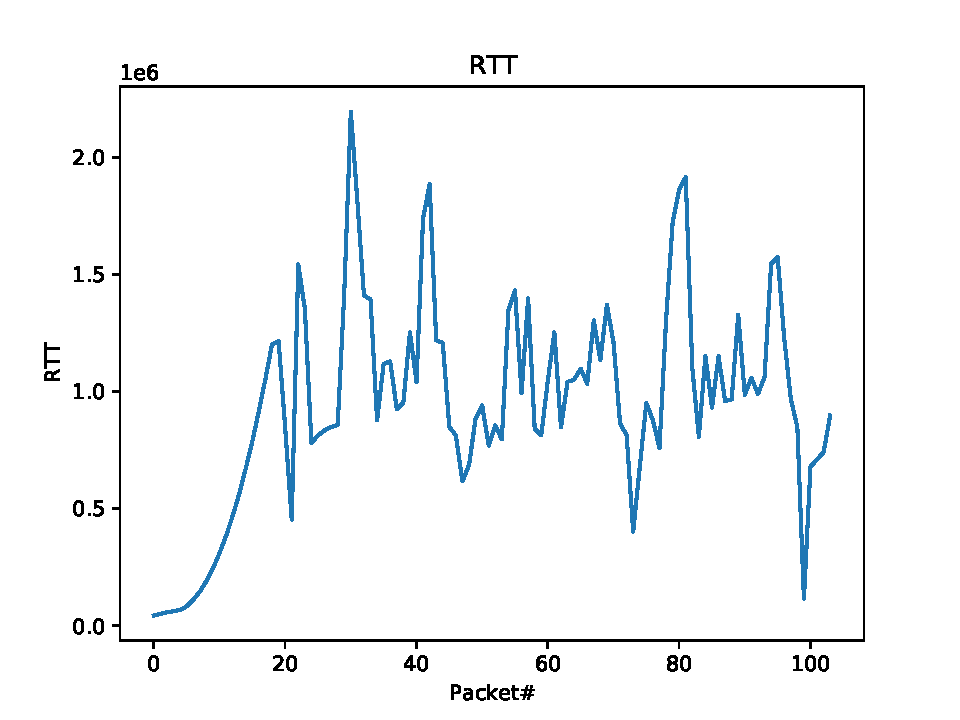
\includegraphics[page=1, width = 0.6 \textwidth]{images/plots.pdf}
\end{center}

\begin{center}
	\includegraphics[page=2, width = 0.6 \textwidth]{images/plots.pdf}
\end{center}

\begin{center}
	\includegraphics[page=3, width = 0.6 \textwidth]{images/plots.pdf}
\end{center}

\end{enumerate}

در مورد تحلیل این نمودارها، با بالارفتن پنجره Congestion شاهد افت‌های ناگهانی آن براساس الگوریتم‌های کنترل Congestion هستیم. در لحظاتی که با Congestion خیلی بالا رو به رو هستیم، مشاهده می‌کنیم که RTT هم بالا رفته است که به معنی کند شدن شبکه است و بلافاصله بعد از کاهش پنجره Congestion شاهد افت شدید RTT هم هستیم که نشان‌دهنده بالا رفتن سرعت شبکه است. از طرف دیگر گذردهی هم در همان لحظاتی که RTT به شدت زیاد شده، با کاهش چشمگیری رو به رو شده است و همچنین در لحظاتی که RTT کاهش چشمگیری داشته و پنجره Congestion کاهش شدید پیدا کرده است و دوباره تنظیم شده، شاهد افزایش شدید  گذردهی در لحظه بعدی هستیم زیرا مواردی که در اثر ازدحام دچار مشکل شده بودند، با خلوت شدن شبکه به راحتی منتقل شده اند. در باقی موارد شاهد رفتار نوسانی نسبتا معقولی در شبکه هستیم و اتفاق شاخصی رخ نمی‌دهد.
\end{document}



